\documentclass[letterpaper, 11pt]{book}

%---------------------Paquetes a utilizar---------------------------%
\usepackage[left=3.6cm,right=2.54cm,top=2.54cm,bottom=2.54cm]{geometry}%Formato general de la página y márgenes 
\usepackage[utf8]{inputenc}                 %Encoding
\usepackage[english]{babel}                 %Español
\usepackage{csquotes}                       %Herramientas para citar
\usepackage[style = ieee]{biblatex}          %Manejo de bibliografía
\usepackage{amsmath}                        %Algunos entornos matemáticos (como align)
\usepackage[labelfont=bf]{caption}          %Formato de figuras
\usepackage{subcaption}                     %subfigures
\usepackage{graphicx}                       %Manejo de imágenes
\usepackage{hyperref}                       %Uso de hipervínculos
\usepackage{titlesec}                       %Para modificar el formato de los títulos
\usepackage{fancyhdr}                       %Encabezados y pie de páginas personalizados
\usepackage{lipsum}
\usepackage{nomencl}
\makenomenclature
\renewcommand{\nomname}{List of symbols and abbreviations}
\usepackage{siunitx}


%---------Configurar algunas propiedades del documento-------------%
%\renewcommand{\baselinestretch}{1.5}        %Interliniado de 1.5   

%\addto\captionsspanish{\renewcommand{\listfigurename}{Lista de figuras}}
%\addto\captionsspanish{\renewcommand{\listtablename}{Lista de tablas}}
%\addto\captionsspanish{\renewcommand{\figurename}{Figura}}
%\addto\captionsspanish{\renewcommand{\tablename}{Tabla}}

%\renewcommand\thefigure{\thechapter-\arabic{figure}}
% \renewcommand\thetable{\thechapter-\arabic{table}}

\def\imagesize{0.8\textwidth}

\renewcommand{\chaptermark}[1]{\markboth{#1}{}}%Definición de cómo se almacena el nombre del capítulo


%-----------Formato de títulos de capítulo--------------------------%
\titleformat{\chapter}[display]
{\normalfont\huge\bfseries}{\chaptertitlename\ \thechapter}{20pt}{\Huge}                                     %Propiedades por defecto de los títulos de capítulo

\titlespacing*{\chapter}{0pt}{100pt}{24pt}  %Dar espaciado de 100pt en la parte superior y 24pt en la parte inferior del título de capítulo

%-------------Formato de pies de página y encabezados---------------%

\fancypagestyle{plain}{
    \fancyhf{}
    \renewcommand{\headrulewidth}{0pt} 
    \renewcommand{\footrulewidth}{0pt}}     %Estilo de la primera página de cada capítulo 



\pagestyle{fancy}
\fancyhf{}
\fancyhead[RE,LO]{\thepage}
\fancyhead[RO,LE]{\leftmark}  


%-----------------Archivo con referencias bibliográficas------------%
\addbibresource{references.bib} % Biblatex


%------------------Inicio del documento-----------------------------%
\begin{document}
\frontmatter

\begin{titlepage}
    \begin{center}
          
      	\begin{figure}[ht]
      		
\includegraphics[width=0.3\textwidth]{images/preliminaries/EscudoUNAL.png}
      		\centering
      	\end{figure}
            
        \vspace{3.5cm}
            
        \LARGE{\textbf{Título del proyecto}}
        
        
        \vspace{3.5cm}
        \large{\textbf{Nombre de xlx estudiante}}
        \vfill
        
        
        \normalsize{Universidad Nacional de Colombia\\
					Facultad de , Departamento \\
					Ciudad, Colombia\\
					Año}
            
    \end{center}
\end{titlepage}
\let\cleardoublepage\clearpage
\begin{titlepage}
    \begin{center}            
        \LARGE{\textbf{Título del proyecto}}  
            
        \vspace{3.5cm}
        \large{\textbf{Nombre de xlx estudiante}}
            
        \vspace{3.5cm}
        \normalsize{Trabajo presentado como requisito parcial para optar al título de:\\
        \textbf{Título esperado}}    
     
        \vspace{2cm}
        \normalsize{Directorx:\\ Nombre de quien dirige}
        
        \vspace{1.2cm}
        \normalsize{L\'inea de Investigaci\'on:\\Línea de investigación}
        \vfill
		\normalsize{Universidad Nacional de Colombia\\
					Facultad de , Departamento de \\
					Ciudad, Colombia\\
					Año}
            
    \end{center}
\end{titlepage}

\setcounter{page}{1}
\chapter*{Acknowledgments}
\chaptermark{Acknowledgments}





\chapter*{Abstract}
\addcontentsline{toc}{chapter}{Abstract} 
\chaptermark{Abstract}




\tableofcontents

\cleardoublepage
\phantomsection
\addcontentsline{toc}{chapter}{\listfigurename} 
\listoffigures

\cleardoublepage
\phantomsection
\addcontentsline{toc}{chapter}{\listtablename} 
\listoftables

\cleardoublepage
\phantomsection
\addcontentsline{toc}{chapter}{\nomname} 
\printnomenclature

\cleardoublepage


\mainmatter
\chapter{Introduction}
\chaptermark{Introduction}
\label{ch:introduction}


	

Square-law detection, also known as Direct detection (DD), is a detection scheme that measures the square magnitude of a complex wave form, clearly this scheme is a nonlinear waveform detection because of the square operation. Direct detection is widely used in different scientific fields, for example in crystallography, radio astronomy, biomedical spectroscopy, among others \cite{Tasbihi_Tukey}. In particular this scheme is often used in optical communications, specially in short-haul systems with length up to \SI{50}{\km} \cite{Agrawal_ch1} due to its simplicity, or even in shorter links up to \SI{10}{\km} for example in rack to rack communications in big data centers.\\
\nomenclature{DD}{Direct Detection}

In the recent years the interest of studying systems with DD is getting bigger again, because of the simplicity of the receivers, which are a promising low-cost alternative compared to the coherent detection systems \cite{Mecozzi_2018}. In this context two questions or problems arise. First, how good is a system with DD compared to a system with coherent detection in terms of the information capacity of the channels. And second, how to design a system that exploits the information capacity of the DD channel in the best possible way.\\

In this work we cover briefly two answers given to the first question, and then we review two systems proposed for a channel with DD. Then we propose a new decoder for the second system, with reduced complexity at the expenses of a slightly worse performance.




\section{Direct Detection}
\label{sec:Direct_Detection}

In optical communication DD is performed with a single photodiode, that convert the optical signal to an electric signal trough the photoelectric effect according to the next equation \cite{Agrawal_ch4}:
\begin{equation}
I_p = R_d\cdot P_{in}
\label{eq:photocurrent}
\end{equation}
where $I_p$ is the photocurrent, $P_{in}$ is the incident optical power (which is proportional to the square of the magnitud of the electric field, that is where the square-law term comes from), and $R_d$ is the so called responsivity of the photodetector, with units of \SI{}{\A/\W}.\\

The noise in the photodiode are generated primarily by two mechanisms, in the first place the shot noise, and in the second place thermal noise.\\

The shot noise is models the fact that the photocurrent consist of a stream of electrons generated at random times. Mathematically the current corresponding to the shot noise $i_s(t)$ is a stationary random process with Poisson distribution, but is usually approximated by a Gaussian distribution with variance given by \cite{Agrawal_ch4}:
\begin{equation}
\sigma_s^2 = 2qI_pB
\label{eq:shot_noise_varaince}
\end{equation}
where $q$ is the electron charge, $I_p$ the photocurrent, and $B$ the bandwidth of the system. $\sigma_s$ can be interpreted as the RMS value of the shot noise current $i_s(t)$.\\ 

The termal noise is generated by the movement  of electrons due to the ambient temperature, and the variance of the noise is given by \cite{Agrawal_ch4}:
\begin{equation}
\sigma_{th}^2 = \frac{4k_BT}{R_L} F_nB
\label{eq:thermal_noise_variance}
\end{equation}
where $k_B$ is the Boltzmann constant, $T$ is the temperature given in kelvin, $R_L$ is the load resistance, $B$ the bandwidth, and $F_n$ is the amplifier noise figure. \\

With this in mind the output current of the direct detection process is given by:
\begin{equation}
I(t) = I_p+i_s(t)+i_{th}(t)
\label{eq:DD_current}
\end{equation}
with $i_s(t)\sim\mathcal{N}(0,\sigma_s^2)$ and $i_{th}(t)\sim\mathcal{N}(0,\sigma_{th}^2)$
\nomenclature{$X\sim\mathcal{N}(\mu,\sigma^2)$}{$X$ has a Gaussian distribution with mean $\mu$ and variance $\sigma^2$}


\section{Capacity under direct detection}
\label{sec:capacity_under_direct_detection}

A communications channel that uses DD can retrieve only the information about the magnitude of the signal, in contrast a system with coherent detection can retrieve the magnitud and phase of the signal. This means that DD scheme ignores one of the two degrees of freedom, and hence it is reasonable to think that the capacity of this systems should be approximately half that of the system with coherent detection \cite{Mecozzi_2018, Tasbihi_Tukey, Tasbihi_Capacity}.\\

However in \cite{Mecozzi_2018} it is shown that the spectra efficiency of a band limited system under DD is at most \SI{1}{bit/\s/\Hz} less than the same system under coherent detection. Also in \cite{Tasbihi_Capacity} it is proven that for time limited signals  the capacity is also at most one bit les than the coherent case. This means that contrary to intuition, the loss in the capacity of a system under DD is not a half of the coherent system, but just \SI{1}{bit/\s/\Hz}.\\

The results of this papers show that the systems with DD have a big potential, because the detector are cheaper and easier to implement (basically just one photodiode) and the loss in the capacity may not be as big as thought. However the problem to find a system simple enough that uses the potential of the DD is still open. 



\section{Basic principle of phase recovery}

The key to retrieve the phase information of the transmitted symbols when using DD is to make use of the ISI. As a toy example one can think on the problem where given two complex numbers $z_1$ and $z_2$, from $|z_1|^2$, $|z_2|^2$ and $|z_1+z_2|^2$ (an ISI term), it is possible to determine the phase difference between $z_1$ and $z_2$ up to a sign ambiguity \cite{Tasbihi_Tukey}.\\

To show this, notice the following:
\begin{align*}
	|z_1+z_2|^2 &= (z_1+z_2)(z_1+z_2)^* \\
	&=z_1z_1^*+z_1z_2^*+z_2z_2^*+z_1^*z_2\\
	&=|z_1|^2+|z_2|^2+z_1z_2^*+\bigl(z_1z_2^*\bigr)^*\\
	&=|z_1|^2+|z_2|^2+2\text{Re}\{z_1z_2^*\}\\
\end{align*}
under the convention that $z_1 = a\cdot e^{j\alpha}$ and $z_2 = b\cdot e^{j\beta}$
\begin{equation}
	|z_1+z_2|^2 =|z_1|^2+|z_2|^2+2|z_1||z_2|\cos(\alpha-\beta)\\
	\label{eq:square_mag_of_sum}
\end{equation}
\nomenclature{$j$}{Imaginary unit}
\nomenclature{Re$\{z\}$}{Real part of $z$}
\nomenclature{Im$\{z\}$}{imaginary part of $z$}

Clearly if $|z_1|^2$, $|z_2|^2$ and $|z_1+z_2|^2$ are known, one can solve the equation \ref{eq:square_mag_of_sum} for $\cos(\alpha-\beta)$ and get the information about the phase difference between $z_1$ and $z_2$. However, since cosine is an even function $\cos(\alpha-\beta)=\cos(-\alpha+\beta)$, hence there is still an ambiguity on the sign of the phase difference.\\


\begin{figure}[htb]
     \centering
     \begin{subfigure}[b]{0.49\textwidth}
         \centering
         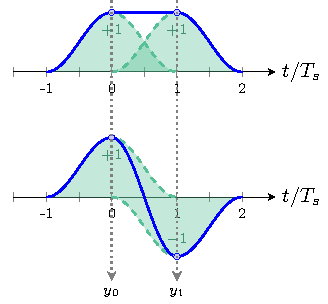
\includegraphics[width=\textwidth]{images/CD_toy_example.pdf}
         \caption{Coherent detection}
         \label{fig:CD_toy_example}
     \end{subfigure}
     \hfill
     \begin{subfigure}[b]{0.49\textwidth}
         \centering
         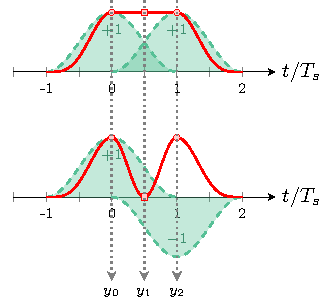
\includegraphics[width=\textwidth]{images/DD_toy_example.pdf}
         \caption{Direct detection}
         \label{fig:DD_toy_example}
     \end{subfigure}
     \hfill
     \vspace{10mm}
     \begin{subfigure}[b]{0.8\textwidth}
         \centering
         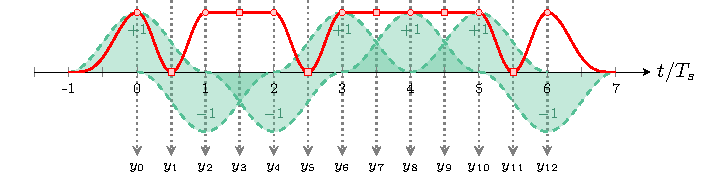
\includegraphics[width=\textwidth]{images/DD_toy_example_long_sq.pdf}
         \caption{Direct detection of the sequence $\{+1,-1,-1,+1,+1,+1,-1\}$}
         \label{fig:DD_toy_example_long_sq}
     \end{subfigure}
        \caption{Comparative of the wave forms under coherent detection and direct detection. Based on \cite{Secondini, Plabst_DD}.}
        \label{fig:DD_vs_CD}
\end{figure}

To visualize this principle in a real system (jet not even near to optimal due to the big bandwidth of the pulse), see the figure \ref{fig:DD_vs_CD}. There is shown with a solid line the wave form of a simple transmission under coherent detection (see figure \ref{fig:CD_toy_example}) and under direct detection (see figure \ref{fig:DD_toy_example}), and also the wave form of the individual symbols in dashed lines.\\

For the coherent detection case the samples at each symbol time are sufficient to determine the transmitted symbols. In contrast, for the direct detection case the samples at each symbol time (circles) only carry information about the magnitude of the symbols (always one in this example); and the samples at intermediate symbol time (squares) carry information about the phase difference \cite{Secondini}.\\

Figure \ref{fig:DD_toy_example_long_sq} show the DD system for a longer sequence, there it is possible to notice that the even samples always carry information about the magnitude, whereas the odd samples carry information about the differential phase of the symbols. This toy example shows the principle behind the phase recovery in DD systems, it is important to highlight two things, first an oversampling factor of two is needed, and second only information on the differential phase (up to a sign ambiguity) is retrieved, hence it is beneficial to use differential coding in the transmission.\\

An other way to explain the previous conclusions is to take a look at the simple system given by:
\begin{align*}
	g(t)=\sum_{k=0}^m g_k\text{sinc}(t-k)
\end{align*}
where $g_k$ is a complex number representing the transmitted symbol and $g(t)$ is the transmitted signal. Note that after the DD the bandwidth of the signal is twice as big as the bandwidth of $g(t)$, since the received signal is given by the product $|g(t)|^2=g(t)g^*(t)$. Hence to recover the data one should use an oversampling factor of two, so the sampled signal becomes \cite{Tasbihi_Tukey}:
\begin{align*}
	\left|g\left(\frac{n}{2}\right)\right|^2 = \left\{
\begin{array}{ll}
\left|g_{\frac{n}{2}}\right|^2  &  \text{if $n$ is even}  \\
\left|\sum\limits_{k=0}^m g_k\text{sinc}\left(\frac{n}{2}-k\right)\right|^2   & \text{if $n$ is odd}
\end{array}
\right. &&\text{for }n=0,\dotsb,2m
\end{align*}
\nomenclature{sinc$(t)$}{$\frac{\sin(\pi t)}{\pi t}$}

Once again, it is clear that the even samples carry the information about the magnitude of the symbols, whereas the odd samples carry some how the information about the phase of the symbols. But now notice that all the $g_k$ contribute to the odd samples, this makes that retrieving the phase becomes quickly an intractable problem as $m$ grows \cite{Tasbihi_Tukey}, as we will see in later chapters. 




















\chapter{Tukey signaling}
\chaptermark{Tukey signaling}
\label{ch:Tukey_signaling}
\newcommand{\TukeyImage}[1]{images/Tukey_Signaling/#1}

	

One of the solutions given to the problem of phase recovery under DD is the so called Tukey signaling proposed in \cite{Tasbihi_Tukey}. The main idea in this paper is to introduce controlled ISI in the transmission and use the interference between symbols to recover the phase of the symbols in a block of length $n$ symbols. The system proposed for shor-haul systems, specifically for links with lengths less than \SI{10}{\km}.\\
  
The system model proposed in the paper is shown in figure \ref{fig:Tukey_system_model}. In the following sections each block will be explain and discussed when needed. Nevertheless the blocks will be explained in a different order, to facilitate understanding. First the dispersion precompensation, the transmission medium and the photodiode will be explained, then the signaling block, integrate and dump, class representative, and finally the decoder.

\begin{figure}[htbp]
\begin{center}
\includegraphics[width=0.8\textwidth]{\TukeyImage{Tukey_system_model.pdf}}
\caption{System model for Tukey signaling. Based on \cite{Tasbihi_Tukey}}
\label{fig:Tukey_system_model}
\end{center}
\end{figure}

\section{System model}
\label{sec:Tukey_system_model}

\subsection{Dispersion precompensation}

In this block the chromatic dispersion of the optical fiber is precompensated, by an all-pass filter with transfer function
\begin{equation}
H(f)=e^{j2\beta_2L\pi^2f^2}
\label{eq:dispersion_precompensation}
\end{equation}
where $\beta_2$ is the group-velocity dispersion parameter and $L$ is the fiber length \cite{Tasbihi_Tukey}.\\

Clearly from this description of the block, the following relations between $x(t)$ and $u(t)$ are given:
\begin{equation}
	u(t)=\mathcal{F}^{-1}\bigl\{X(f)H(f)\bigr\}
	\label{eq:Tuey_Disp_precomp}
\end{equation}
where $X(f)$ is the Fourier transform of $x(t)$

\nomenclature{$f$}{Frequency}
\nomenclature{$\mathcal{F}\{\cdot\}$}{Fourier transform }
\nomenclature{$\mathcal{F}^{-1}\{\cdot\}$}{Inverse fourier transform }

\subsection{Transmission medium}

Since the optical fiber length is less than \SI{10}{\km} it is possible to ignore all the transmission impairments, except for power loss and chromatic dispersion \cite{Tasbihi_Tukey}. With this in mind, and taking into account the dispersion pre compensation, we have the following relation:
\begin{equation}
r(t)=\rho x(t)
\label{eq:Tukey_fiber_out}
\end{equation}
 where $0<\rho\leq1$ is the attenuation constant, that depends on the length of the fiber. The spacial case $\rho=1$, i.e. without attenuation, is called back-to-back transmission.

\subsection{Photodiode}

For this system an avalanche photodiode (APD) is used, and this diode is considered as the only source of noise. In this case both shoot and thermal noise are considered. The behavior of  the diode is given by \cite{Tasbihi_Tukey}:
\begin{equation}
s(t)=\bigl|r(t)\bigr|^2+\bigl|r(t)\bigr|n_{sh}(t)+n_{th}(t)
\label{eq:Tukey_PD}
\end{equation}
where $n_{sh}(t)$ and $n_{th}(t)$ are gaussian distributed and the variance of each noise is given by \cite{Tasbihi_Tukey}:
\begin{align}
	\sigma^2_{th}&=\frac{4k_BTB}{R_L}\\
	\sigma^2_{sh}&=2qM^2_{\text{APD}}FR_\text{APD}B
\end{align}

Notice that the difference of between the $\sigma^2_{sh}$ presented here and the equation \ref{eq:shot_noise_varaince} is due to the gain of the APD.

\subsection{Signaling}

This block receive $n$ complex numbers $x_0,\dotsc,x_{n-1}$, which are the transmitted symbols, and produces continuous time complex signal given by:
\begin{equation}
x(t)=\sum_{i=0}^{n-1}x_iw(t-iT)
\label{eq:Tukey_signaling_block}
\end{equation}
where $T$ is the inverse of the baud rate and $w(t)$ is a wave form.\\

Usually in communications $w(t)$ is a root raised-cosine waveform, however the ISI of this pulse at times different to the symbol time is to complicated, because a lot of symbols interfere if not all of them, and that make the problem of recovering the phase to complicated. That is why in the paper is proposed a time limited waveform with a simpler ``ISI pattern''.

The proposed waveform is the Tukey window, which is equivalent to the Fourier transform of a raised-cosine but in time domain.
This waveform is given by:
\begin{align}
	w_\beta(t)&=\left\{
\begin{array}{ll}
 \frac{2}{\sqrt{4-\beta}} & \text{if } |t|\leq\frac{1-\beta}{2}\\
 \frac{1}{\sqrt{4-\beta}}\left(1-\sin\left(\frac{\pi(2|t|-1)}{2\beta}\right)\right)&\text{if } \left||t|-\frac{1}{2}\right|\leq\frac{\beta}{2}\\
  0&\text{otherwise}  
\end{array}
\right.
\label{eq:Tukey_window_TD}\\
W_\beta(f)&=\left\{
\begin{array}{ll}
  \frac{\pi}{2\sqrt{4-\beta}}\cdot\text{sinc}\left(\frac{1}{2\beta}\right)&\text{if } f=\pm\frac{1}{2\beta}\\
  \frac{2}{\sqrt{4-\beta}}\cdot\text{sinc}(f)\cdot\frac{\cos(\pi\beta f)}{1-(2\beta f)^2}&\text{otherwise}   
\end{array}
\right.
\label{eq:Tukey_window_FD}
\end{align}
Notice that the factor $2/\sqrt{4-\beta}$ is to normalize the energy of the waveform.\\

The waveform can be seen in figure \ref{fig:Tukey_window} both in time domain and frequency domain for two different $\beta$. 
\begin{figure}[htb]
     \centering
     \begin{subfigure}[b]{0.8\textwidth}
         \centering
         \includegraphics[width=\textwidth]{\TukeyImage{Tukey_window_TD.pdf}}
         \caption{Time domain}
         \label{fig:Tukey_window_TD}
     \end{subfigure}
     \hfill
     \begin{subfigure}[b]{0.8\textwidth}
         \centering
         \includegraphics[width=\textwidth]{\TukeyImage{Tukey_window_FD.pdf}}
         \caption{Frequency domain}
         \label{fig:Tukey_window_FD}
     \end{subfigure}
     \hfill
     \caption{Tukey window for different $\beta$, $\beta_1<\beta_2$. Based on \cite{Tasbihi_Tukey}}
     \label{fig:Tukey_window}
\end{figure}

When we select $w(t)=w_\beta(t/T)$ in equation \ref{eq:Tukey_signaling_block}, the resulting signal have an important property: 
at any given time, either only one or only two symbols contribute to the value of the signal, here we see the meaning of \textit{controlled} ISI. According to this property we define two types of intervals, an ISI-free interval $\mathcal{Y}_i$, where $x(t)$ depends only on $x_i$; and an ISI-present interval $\mathcal{Z}_i$, where $x(t)$ depends only on $x_i$ and $x_{i+1}$. Those intervals are shown in the figure \ref{fig:Tukey_ISI} and are given by:
\begin{align}
	\mathcal{Y}_i&: \left[\left(i-\frac{1-\beta}{2}\right)T, \left(i+\frac{1-\beta}{2}\right)T\right] && i\in \{0,\dotsc,n-1\}\\
	\mathcal{Z}_i&: \left[\left(i+\frac{1-\beta}{2}\right)T, \left(i+\frac{1+\beta}{2}\right)T\right] && i\in \{0,\dotsc,n-2\}
\end{align}

\begin{figure}[htbp]
\begin{center}
\includegraphics[width=0.9\textwidth]{\TukeyImage{Tukey_ISI.pdf}}
\caption{ISI-free and ISI-pressent intervals for $n=3$}
\label{fig:Tukey_ISI}
\end{center}
\end{figure}

Other consequence of choosing this wave form is that, in frequency domain, the signal is not band limited, however the amplitude of $W_\beta(f)$ tends to 0 as the frequency increase, so it is possible to define the bandwidth of the waveform as the smallest interval containing the 95\% of the signal energy \cite{Tasbihi_Tukey}. With this definition we get the bandwidths seen in table \ref{tab:BW_Tukey_window} for different $\beta$.

\begin{table}[htp]
\begin{center}
\begin{tabular}{|c|c|c|}\hline
$\beta$&Bandwith [\SI{}{\Hz}]&overhead\\\hline
0.1&1.477&195.4\%\\\hline
0.3&0.788&57.6\%\\\hline
0.5&0.668&33.6\%\\\hline
0.7&0.613&22.6\%\\\hline
0.8&0.592&18.4\%\\\hline
0.9&0.575&15.0\%\\\hline
\end{tabular}
\end{center}
\caption{Bandwidth containing 95\%of the waveform energy, and the overhead compared to the minimum bandwidth for Nyquist signaling. Taken from \cite{Tasbihi_Tukey}}
\label{tab:BW_Tukey_window}
\end{table}%

\subsection{Integrate and dump}

This block integrate the incoming signal $s(t)$ in the different intervals $\mathcal{Y}_i$ and $\mathcal{Z}_i$ to produce the real valued samples $y_i$ and $z_i$ given by:
\begin{align}
	y_i&=\int_{\mathcal Y_i}s(t)dt&&i\in \{0,\dotsc,n-1\}\\
	z_i&=\int_{\mathcal Z_i}s(t)dt&&i\in \{0,\dotsc,n-2\}
\end{align}

It can be shown that $y_i$ is given by \cite{Tasbihi_Tukey}:
\begin{equation}
y_i=\alpha^2(1-\beta)T|x_i|^2+\alpha|x_i|n_i+m_i
	\label{eq:y_i_Tukey}
\end{equation}
where $\alpha=2/\sqrt{4-\beta}$, $n_i\sim\mathcal N(0,\sigma^2_{sh}(1-\beta)T)$ and $m_i\sim\mathcal N(0,\sigma^2_{th}(1-\beta)T)$.\\

Also defining:
\begin{align}
\psi(v,w)&=\frac{1}{4}|v+w|^2 + \frac{1}{8}|v-w|^2
\end{align}
which can be expanded using equation \ref{eq:square_mag_of_sum} as:
\begin{align}
\psi(ae^{j\alpha},be^{j\beta})&=\frac{3}{8}\left(a^2+b^2\right)+\frac{1}{4}ab\cos(\alpha-\beta)
\end{align}
 it is possible to show that $z_i$ is given by \cite{Tasbihi_Tukey}:
\begin{equation}
	z_i=\alpha^2\beta T\psi(x_i,x_{i+1})+\alpha\sqrt{\psi(x_i,x_{i+1})}p_i +q_i
	\label{eq:z_i_Tukey}
\end{equation}
where $p_i\sim\mathcal N(0,\sigma^2_{sh}\beta T)$ and $q_i\sim\mathcal N(0,\sigma^2_{th}\beta T)$.\\

Notice that $n_i$, $m_i$, $p_i$ and $q_i$ are mutually  independent, and that all the $y_i$ carry information about the magnitude of the transmitted symbols, and all the $z_i$ carry information about the interface between adjacent symbols, i.e. the phase difference between symbols.

\subsection{Class representative}

When transmitting symbol blocks ($n$ consecutive symbols) it turns out that there are some ambiguities, that means that two different symbol blocks produces the same output of the system. Of course we want to avoid this situation to achieve a reliable communication, and that is what the Class representative block of figure \ref{fig:Tukey_system_model} does.\\

To formalize the problem let define the function $\Upsilon: \mathds{C}^n\to(\mathds{R}^n,\mathds{R}^{n-1})$ that maps a vector $\bm x$ at the input of the signaling block, to the output of the integrate and dump block, in the absence of noise \cite{Tasbihi_Tukey}. That means:
\begin{align}
	\Upsilon(\bm x) = (\bm y, \bm z)
\end{align}
where $\bm x\in\mathds{C}^n$, $\bm y\in\mathds{R}^n$, $\bm z\in\mathds{R}^{n-1}$ and 
\begin{align}
	y_i&=\int_{\mathcal Y_i}\bigl|x(t)\bigr|^2dt&&i\in \{0,\dotsc,n-1\}\\
	z_i&=\int_{\mathcal Z_i}\bigl|x(t)\bigr|^2dt&&i\in \{0,\dotsc,n-2\}
\end{align}

Now we define an equivalence relation in $\mathds C^n$, where two vectors $\bm x$ and $\bm{\tilde{x}}$ are square law equivalent if and only if $\Upsilon(\bm x)=\Upsilon(\bm{\tilde{x}})$, and we denote the equivalence by $\bm x \equiv \bm{\tilde{x}}$ \cite{Tasbihi_Tukey}.\\

The Class representative block consist of a set $\mathcal S$ of cardinality $M$, whose elements belong to $\mathds{C}^n$ and are all square law distinct \cite{Tasbihi_Tukey}, that is:
\begin{align}
	\mathcal S = \{\bm x_1, \dotsc,\bm x_M\} \subset\mathds C^n\qquad \text{such that}\qquad\bm x_i\not\equiv\bm x_l \Leftrightarrow k\neq l
\end{align}
and for an input $k\in\{1,\dotsc,M\}$ the block outputs $\bm x_k$ \cite{Tasbihi_Tukey}:
\begin{align}
	k& \longrightarrow\text{Class Representative}\longrightarrow \bm x_k && k\in\{1,\dotsc,M\}
\end{align} 

Notice that this scheme, can transmit $M$ different symbol blocks using $n$ symbols, thus the spectral efficiency of this channel can not exceed $\frac{1}{n}\log_2(M)\SI{}{bits/\s/\Hz}$ \cite{Tasbihi_Tukey}.

\subsubsection{Analysis on ambiguities}

There are two key points to understand the origin of the ambiguities. The first, and most important, is to notice that the detection of a symbol block is based only on the information about the magnitude of each symbol (present on each $y_i$) and the information about the phase difference between adjacent symbols (present on each $z_i$). That means that every two vectors whose elements have the same magnitude, and the phase difference between adjacent elements is the same, are square law equivalent.\\

The second key point is to notice that the symbols of the symbol blocks belong to a constellation $\mathcal K$ (some examples of possible constellation are shown on figure \ref{fig:constellations_Tukey}), that means that a $\bm x\in \mathcal K^n \subset\mathds{C}^n$, in other words $\bm x$ belongs to a finite subset of $\mathds{C}^n$.\\

Summarizing, all $n$-tuple of points in a given constellation that have the same magnitudes and same phase difference between adjacent symbols are square law equivalent and generate ambiguities. Lets define equivalence class as the set of all such vectors, so an equivalence class $\mathcal{E}$ of size $L$ is given by:
\begin{align}
	\mathcal E=\{\bm x_1, \dotsc,\bm x_L\} \subset\mathds C^n\qquad \text{such that}\qquad\bm x_i\equiv\bm x_j\quad \forall i,j \in \{1,\dotsc,L\} 
\end{align}


\begin{figure}[htb]
     \centering
     \begin{subfigure}[b]{0.4\textwidth}
         \centering
         \includegraphics[width=\textwidth]{\TukeyImage{Eq_class_construction_0.pdf}}
         \caption{}
         \label{fig:Eq_class_construction_0}
     \end{subfigure}
     \hspace{10mm}
     \begin{subfigure}[b]{0.4\textwidth}
         \centering
         \includegraphics[width=\textwidth]{\TukeyImage{Eq_class_construction_1.pdf}}
         \caption{}
         \label{fig:Eq_class_construction_1}
     \end{subfigure}
     \hfill
     \begin{subfigure}[b]{0.4\textwidth}
         \centering
         \includegraphics[width=\textwidth]{\TukeyImage{Eq_class_construction_2.pdf}}
         \caption{}
         \label{fig:Eq_class_construction_2}
     \end{subfigure}
     \hspace{10mm}
     \begin{subfigure}[b]{0.4\textwidth}
         \centering
         \includegraphics[width=\textwidth]{\TukeyImage{Eq_class_construction_3.pdf}}
         \caption{}
         \label{fig:Eq_class_construction_3}
     \end{subfigure}
     \hfill
     \caption{Construction of 4 different but square law equivalent symbol blocks.}
     \label{fig:Eq_class_construction_4base}
\end{figure}

To understand better the equivalence classes, lets look an example of equivalence class when the symbol block length is $n=4$ and the constellation is a 5-ring 5-ary phase (see figure \ref{fig:5ring5ary_phase}) and how to construct it.\\

The first step is to select 4 random points of the constellation to create a symbol block. Take for example the points shown in the figure \ref{fig:Eq_class_construction_0}, there the transmitted symbols are the vertices of the graph, and the order of transmission is given by the small number in each point.\\

Now to create a new equivalent symbol block one can reflect the third and fourth symbol along the symmetry axis that pass through the second symbol, as shown in the figure \ref{fig:Eq_class_construction_1}. Notice that the firs and second symbols do not change, hence their magnitudes are the same, and the phase difference between they also. The third and fourth symbols change, but since the symmetry axis passes through the origin their magnitudes do not change, and neither does the phase difference between them. The phase difference between the second and third symbol in both symbol blocks is also the same as shown in figure \ref{fig:Eq_class_construction_1}. Finally, all the points of the new symbol block lay on a valid constellation point, due to the high symmetry of the constellation. Hence the first symbol block and the new one are valid (belong to $\mathcal K^4$) and square law equivalent so they belong to the same equivalence class.\\

The same process can be applied to the fourth symbol, and using as symmetry axis the axis that passes trough the third symbol as shown in the figure \ref{fig:Eq_class_construction_2}. Using the same arguments the new symbol block is equivalent to the previous two and belongs to the same equivalence class. Now from this new symbol block, reflecting the third and fourth symbol as shown in the figure \ref{fig:Eq_class_construction_3} one can create a new fourth symbol block that belongs to the same equivalence class.\\

Now we have 4 different, but square law equivalent symbol blocks, clearly if we reflect all the 4 symbols blocks along the real axis, we create 4 new different symbol blocks that belong to the equivalence class, as shown in figure \ref{fig:Eq_class_construction_reflection}.\\

\begin{figure}[htb]
     \centering
     \begin{subfigure}[b]{0.24\textwidth}
         \centering
         \includegraphics[width=\textwidth]{\TukeyImage{Eq_class_construction_4.pdf}}
         \caption{}
         \label{fig:Eq_class_construction_4}
     \end{subfigure}
     \hfill
     \begin{subfigure}[b]{0.24\textwidth}
         \centering
         \includegraphics[width=\textwidth]{\TukeyImage{Eq_class_construction_5.pdf}}
         \caption{}
         \label{fig:Eq_class_construction_5}
     \end{subfigure}
     \hfill
     \begin{subfigure}[b]{0.24\textwidth}
         \centering
         \includegraphics[width=\textwidth]{\TukeyImage{Eq_class_construction_6.pdf}}
         \caption{}
         \label{fig:Eq_class_construction_6}
     \end{subfigure}
     \hfill
     \begin{subfigure}[b]{0.24\textwidth}
         \centering
         \includegraphics[width=\textwidth]{\TukeyImage{Eq_class_construction_7.pdf}}
         \caption{}
         \label{fig:Eq_class_construction_7}
     \end{subfigure}
     \hfill
     \caption{Construction of 4 new different but square law equivalent symbol blocks by reflection.}
     \label{fig:Eq_class_construction_reflection}
\end{figure}

Finally we can rotate all the 8 different, but square law equivalent symbol blocks, 4 times around the origin to create 32 new different symbol blocks that belong to the equivalence class, as shown in figure \ref{fig:Eq_class_construction_rotation}. As a result we get all the symbol block that belong to the same equivalence class, those symbol blocks are shown on figure \ref{fig:Eq_class_construction_16}.\\

When looking all the symbol blocks of the equivalence class (see figure \ref{fig:Eq_class_construction_16}), it is possible to notice the high symmetry of the plot, this shows that constellations with high symmetry allow a lot of ambiguities and reduce the achievable rate of the system.


\begin{figure}[htb]
     \centering
     \begin{subfigure}[b]{0.24\textwidth}
         \centering
         \includegraphics[width=\textwidth]{\TukeyImage{Eq_class_construction_8.pdf}}
         \caption{}
         \label{fig:Eq_class_construction_8}
     \end{subfigure}
     \hfill
     \begin{subfigure}[b]{0.24\textwidth}
         \centering
         \includegraphics[width=\textwidth]{\TukeyImage{Eq_class_construction_9.pdf}}
         \caption{}
         \label{fig:Eq_class_construction_9}
     \end{subfigure}
     \hfill
     \begin{subfigure}[b]{0.24\textwidth}
         \centering
         \includegraphics[width=\textwidth]{\TukeyImage{Eq_class_construction_10.pdf}}
         \caption{}
         \label{fig:Eq_class_construction_10}
     \end{subfigure}
     \hfill
     \begin{subfigure}[b]{0.24\textwidth}
         \centering
         \includegraphics[width=\textwidth]{\TukeyImage{Eq_class_construction_11.pdf}}
         \caption{}
         \label{fig:Eq_class_construction_11}
     \end{subfigure}
     \hfill
     \begin{subfigure}[b]{0.24\textwidth}
         \centering
         \includegraphics[width=\textwidth]{\TukeyImage{Eq_class_construction_12.pdf}}
         \caption{}
         \label{fig:Eq_class_construction_12}
     \end{subfigure}
     \hfill
     \begin{subfigure}[b]{0.24\textwidth}
         \centering
         \includegraphics[width=\textwidth]{\TukeyImage{Eq_class_construction_13.pdf}}
         \caption{}
         \label{fig:Eq_class_construction_13}
     \end{subfigure}
     \hfill
     \begin{subfigure}[b]{0.24\textwidth}
         \centering
         \includegraphics[width=\textwidth]{\TukeyImage{Eq_class_construction_14.pdf}}
         \caption{}
         \label{fig:Eq_class_construction_14}
     \end{subfigure}
     \hfill
     \begin{subfigure}[b]{0.24\textwidth}
         \centering
         \includegraphics[width=\textwidth]{\TukeyImage{Eq_class_construction_15.pdf}}
         \caption{}
         \label{fig:Eq_class_construction_15}
     \end{subfigure}
     \hfill
     \caption{Construction of 4 new different but square law equivalent symbol blocks by rotation.}
     \label{fig:Eq_class_construction_rotation}
\end{figure}


\begin{figure}[!h]
\begin{center}
\includegraphics[width=0.5\textwidth]{\TukeyImage{Eq_class_construction_16.pdf}}
\caption{All the symbol blocks in an equivalence class shown at the same time}
\label{fig:Eq_class_construction_16}
\end{center}
\end{figure}




\subsection{Detector}

For the detection, the maximum-likelihood (ML) criterion is chosen, that means that from $\bm y=(y_0,\dotsc,y_{n-1})$  and $\bm z=(z_0,\dotsc,z_{n-2})$, the detector outputs $\hat{k}$ if and only if \cite{Tasbihi_Tukey}:
\begin{equation}
\hat{k}=\argmax_{d\in\{1,\dotsc,M\}}f\bigl(\bm y,\bm z|\bm x_d\bigr)
\label{eq:Tukey_ML}
\end{equation}

Where the PDF of $\bm y,\bm z$ given $\bm x_d$ is given by \cite{Tasbihi_Tukey}:
\begin{equation}
	f\bigl(\bm y,\bm z|\bm x_d\bigr) = f\bigl(\bm y|\bm x_d\bigr)f\bigl(\bm z|\bm x_d\bigr)=\prod_{i=0}^{n-1}f\bigl(y_i|\bm x_d[i]\bigr)\prod_{i=0}^{n-2}f\bigl(z_i|\bm x_d[i],\bm x_d[i+1]\bigr)
\end{equation}

From equations \ref{eq:y_i_Tukey} and \ref{eq:z_i_Tukey} it is clear that $y_i$ and $z_i$ given $x_i$ and $x_{i+1}$ are distributed as \cite{Tasbihi_Tukey}:
\begin{align}
	y_i&\sim\mathcal N \left(\alpha^2(1-\beta)T|x_i|^2,(1-\beta)T(\alpha^2|x_i|^2\sigma^2_{sh}+\sigma^2_{th})\right)\\
	z_i&\sim\mathcal N \left(\alpha^2\beta T\psi(x_i,x_{i+1}),\beta T(\alpha^2\psi(x_i,x_{i+1})\sigma^2_{sh}+\sigma^2_{th})\right)
\end{align}

\nomenclature{PDF}{Probability density function}









\section{Numerical simulation}


\subsection{System parameters}

For the numerical simulation the system is simulated in base band, the baud rate is \SI{10}{Gb/s}, no attenuation in the optical fiber is considered, and the parameter of the diode are taken from \cite{Tasbihi_Tukey} and can be seen on table \ref{tab:diode_Tukey}.\\

\begin{table}[htp]
\begin{center}
\begin{tabular}{|c|c|c|}\hline
Parameter&Value&Typical range\\\hline
Temperature ($T$)&\SI{300}{K}&\\\hline
Load resistance ($R_L$)&\SI{15}{\ohm}&\\\hline
APD Gain ($M_\text{APD}$)&20&10 - 40\\\hline
Enhanced Responsivity ($M_\text{APD}R_\text{APD}$)& \SI{10}{\mA/\mW}& 5 - 20\\\hline
$k$-factor ($k_\text{APD}$)&0.6&0.5 - 0.7\\\hline
Excess noise factor ($F$)&12.78&a function of $M_\text{APD}$ and $k_\text{APD}$\\\hline
\end{tabular}
\end{center}
\caption{Parameter of the photodiode used in the simulations. Taken from \cite{Tasbihi_Tukey}}
\label{tab:diode_Tukey}
\end{table}%

\subsection{Class representative creation}

To define the Class representative block one have to specify a constellation and a block length $n$, then look for all the equivalence classes exhaustively, to finally select one random symbol block from each equivalence class to conform the class representative. In this step several constellations are considered with different block length, six examples of constellations are shown in figure \ref{fig:constellations_Tukey}.\\

To calculate those equivalence classes we use a Python script, that is available on the GitHub repository \href{https://github.com/dfigueroa11/Direct_detection_under_Tukey_Signaling.git}{Direct\_detection\_under\_Tukey\_Signaling}, all the related codes are in the folder \textbf{Equivalence\_classes}. From this code we get all the equivalence classes for the studied constellations and block length, the summary can be seen in the tables \ref{tab:Eq_class_4PSK} to \ref{tab:Eq_class_810ring_810ary} that show the number of equivalence classes sorted by the class size $L$ and the total of equivalence classes for different block lengths $n$, finally is also shown the rate loss, calculated as:
\begin{equation}
R_\text{loss}=\frac{1}{n}\log_2\left(\frac{|\mathcal K|^n}{N_\text{Eq class}}\right)
\label{eq:rate_loss}
\end{equation}
where $|\mathcal K|$ denotes the number of points of the constellation, and $N_\text{Eq class}$ the total of equivalence classes.\\


\begin{figure}[!htb]
     \centering
     \begin{subfigure}[b]{0.32\textwidth}
         \centering
         \includegraphics[width=0.8\textwidth]{\TukeyImage{constellations_4PSK.pdf}}
         \caption{4-PSK}
         \label{fig:4PSK}
     \end{subfigure}
     \hfill
     \begin{subfigure}[b]{0.32\textwidth}
         \centering
         \includegraphics[width=0.8\textwidth]{\TukeyImage{constellations_2ring4ary_phase.pdf}}
         \caption{2-ring 4-ary phase}
         \label{fig:2ring4ary_phase}
     \end{subfigure}
     \hfill
     \begin{subfigure}[b]{0.32\textwidth}
         \centering
         \includegraphics[width=0.8\textwidth]{\TukeyImage{constellations_4ring4ary_phase.pdf}}
         \caption{4-ring 4-ary phase}
         \label{fig:4ring4ary_phase}
     \end{subfigure}
     \hfill
     \begin{subfigure}[b]{0.32\textwidth}
         \centering
         \includegraphics[width=0.8\textwidth]{\TukeyImage{constellations_5ring5ary_phase.pdf}}
         \caption{5-ring 5-ary phase}
         \label{fig:5ring5ary_phase}
     \end{subfigure}
     \hfill
     \begin{subfigure}[b]{0.32\textwidth}
         \centering
         \includegraphics[width=0.8\textwidth]{\TukeyImage{constellations_8ring8ary_phase.pdf}}
         \caption{8-ring 8-ary phase}
         \label{fig:8ring8ary_phase}
     \end{subfigure}
     \hfill
     \begin{subfigure}[b]{0.32\textwidth}
         \centering
         \includegraphics[width=0.8\textwidth]{\TukeyImage{constellations_10ring10ary_phase.pdf}}
         \caption{10-ring 10-ary phase}
         \label{fig:10ring10ary_phase}
     \end{subfigure}
     \hfill
     \hfill
     \caption{Different possible constellations $\mathcal K$.}
     \label{fig:constellations_Tukey}
\end{figure}






\begin{table}[htb]
\begin{center}
\begin{tabular}{|r|m{10mm}<{\raggedleft}|m{10mm}<{\raggedleft}|m{10mm}<{\raggedleft}|m{10mm}<{\raggedleft}|m{10mm}<{\raggedleft}|m{10mm}<{\raggedleft}|}\hline
\backslashbox{Class size}{Block length}&3&4&5&6&7&8\\\hline
4&4&8&16&32&64&128\\
8&4&12&32&80&192&448\\
16&1&6&24&80&240&672\\
32&&1&8&40&160&560\\
64&&&1&10&60&280\\
128&&&&1&12&84\\
256&&&&&1&14\\
512&&&&&&1\\\hline
Total&9&27&81&243&729&2187\\\hline
Rate loss (bit/sym)&0.94&0.81&0.73&0.68&0.64&0.61\\\hline
\end{tabular}
\end{center}
\caption{Number of equivalence classes for 4-PSK constellation.}
\label{tab:Eq_class_4PSK}
\end{table}%


\begin{table}[htb]
\begin{center}
\begin{tabular}{|r|m{10mm}<{\raggedleft}|m{10mm}<{\raggedleft}|m{10mm}<{\raggedleft}|m{10mm}<{\raggedleft}|m{10mm}<{\raggedleft}|}\hline
\backslashbox{Class size}{Block length}&3&4&5&6&7\\\hline
4&32&128&512&2048&8192\\
8&32&192&1024&5120&24576\\
16&8&96&768&5120&30720\\
32&&16&256&2560&20480\\
64&&&32&640&7680\\
128&&&&64&1536\\
256&&&&&128\\\hline
Total&72&432&2592&15552&93312\\\hline
Rate loss (bit/sym)&0.94&0.81&0.73&0.68&0.64\\\hline
\end{tabular}
\end{center}
\caption{Number of equivalence classes for 2-ring 4-ary Phase constellation.}
\label{tab:Eq_class_2ring_4ary}
\end{table}%



\begin{table}[htb]
\begin{center}
\begin{tabular}{|r|m{10mm}<{\raggedleft}|m{10mm}<{\raggedleft}|}\hline
\backslashbox{Class size}{Block length}&3&4\\\hline
5&125&625\\
10&500&3750\\
20&500&7500\\
40&&5000\\\hline
Total&1125&16875\\\hline
Rate loss (bit/sym)&1.27&1.13\\\hline
\end{tabular}
\end{center}
\caption{Number of equivalence classes for 5-ring 5-ary Phase constellation.}
\label{tab:Eq_class_5ring_5ary}
\end{table}%




\begin{table}[!h]
     \centering
     \begin{subtable}[b]{0.4\textwidth}
\begin{center}
\begin{tabular}{|r|m{10mm}<{\raggedleft}|}\hline
\backslashbox{Class size}{Block length}&3\\\hline
8&512\\
16&3584\\
32&6272\\
Total&10368\\\hline
Rate loss (bit/sym)&1.55\\\hline
\end{tabular}
\end{center}
\caption{8-ring 8-ary Phase}
\label{tab:Eq_class_8ring_8ary}


     \end{subtable}
     \hspace{10mm}
     \begin{subtable}[b]{0.4\textwidth}
\begin{center}
\begin{tabular}{|r|m{10mm}<{\raggedleft}|}\hline
\backslashbox{Class size}{Block length}&3\\\hline
10&100\\
20&9000\\
40&20250\\
Total&30250\\\hline
Rate loss (bit/sym)&1.68\\\hline
\end{tabular}
\end{center}
\caption{ 10-ring 10-ary Phase}
\label{tab:Eq_class_10ring_10ary}


     \end{subtable}
     \hfill
     \caption{Number of equivalence classes for different constellations.}
     \label{tab:Eq_class_810ring_810ary}
\end{table}

\subsection{Mutual information estimation}

One of the figure of merit of the system is the Mutual information $I$ of the channel which is given by \cite{MacKay}:
\begin{equation}
I=\sum_{x,y}P(x,y)\log_2\left(\frac{P(x,y)}{P(x)P(y)}\right)
\label{eq:mutual_information}
\end{equation}

To estimate the mutual information we use a Python script to implement a Montecarlo  simulation with \SI{100000}{} symbol blocks (code available on the GitHub repository \href{https://github.com/dfigueroa11/Direct_detection_under_Tukey_Signaling.git}{Direct\_detection\_under\_Tukey\_Signaling}, in the folder \textbf{skripts} file \textbf{main.py}). In this case for the simulation all the possible square law distinct symbol blocks are used.\\

For the 2-ring 4-ary phase constellation and symbol block length $n=3$ we simulated for 4 different $\beta$, and get the results shown in figure \ref{fig:Tukey_result_MI}. Notice that for midium and high SNR the best choice of beta is $\beta=0.9$, also is important to observe that the mutual information tends to  \SI{2,06}{bit/sym} approximately, which is coherent with the rate loss calculated (see table \ref{tab:Eq_class_2ring_4ary})  $$\SI{2.06}{bit/sym}=\SI{3}{bit/sym}-\SI{0.94}{bit/sym}$$

Also is important to notice that the obtained results are coherent with the results reported by \cite{Tasbihi_Tukey}, which show that the implementation of the system made by us is well done.

\begin{figure}[htbp]
\begin{center}
\includegraphics[width=0.9\textwidth]{\TukeyImage{Tukey_result_MI.pdf}}
\caption{Mutual information of the system with 2-ring 4-ary phase constellation and symbol block length $n=3$.}
\label{fig:Tukey_result_MI}
\end{center}
\end{figure}



\subsection{BER estimation}

To estimate the BER, once again a Montecarlo simulation is used, but this time not all the square law distinct symbols are used, instead we use the biggest power of two \cite{Tasbihi_Tukey}. For example for the 2-ring 4-ary phase constellation and symbol block length $n=4$ we use 256 square law distinct symbol blocks instead of 432.\\

Again we simulated for different $\beta$, the 2-ring 4-ary phase constellation and symbol block length $n=4$ to get the results shown in figure \ref{fig:Tukey_result_BER}. The results show the typical behavior of a BER vs SNR graph, again the case of $\beta=0.9$ have the best performance, and the results are coherent with the ones presented by \cite{Tasbihi_Tukey}. 

\begin{figure}[htbp]
\begin{center}
\includegraphics[width=0.9\textwidth]{\TukeyImage{Tukey_result_BER.pdf}}
\caption{Mutual information of the system with 2-ring 4-ary phase constellation and symbol block length $n=4$.}
\label{fig:Tukey_result_BER}
\end{center}
\end{figure}


\section{Discussion}


% discussion 
	% Complexity 
	% bandwidth efficiency 
	% analog circuit may be difficult to implement 

After implementing the system of Tukey signaling, we noticed that the system, at least in simulation, and an ideal situation should work good and is able to retrieve some information about the phase of the complex symbols using only DD. However there are 3 down sides of the system: the complexity of the decoder, the bandwidth efficiency and the implementation.\\

To decrease the rate loss in this system one can increase the block length, but the number of equivalence classes grows exponentially with the block length, and so does the complexity of the decoder, that is why the system becomes impractical really quickly, that is why the complexity of the decoder is a big drawback of the system.\\

An other drawback is the bandwidth efficiency, since the Tukey signal is time limited, its bandwidth is in theory unlimited, and in practice really big compared to others wave forms, such as a sinc pulse. To solve this problem one should increase the duration of the pulse, but doing so the idea of the integrate and dump block is no longer valid, because at some points in time  more than 2 symbols may influence the signal, and the idea of the system was based on the assumption that any time at most 2 symbols influence the signal.\\

Finally the integrate and dump is an analog block by default, which may be complicated to implement, and a digital approximation of the block requires a big oversampling factor which is to expensive in terms of the hardware to do that.\\

For this three drawbacks we decide to look for other solutions in the literature and we stop the work with the system proposed by Tasbihi in \cite{Tasbihi_Tukey}.





































\cleardoublepage
\phantomsection
\addcontentsline{toc}{chapter}{\bibname} 
\printbibliography



\end{document}
